\documentclass[a4paper,11pt, titlepage]{extarticle}

\usepackage{amsmath}
\usepackage{amssymb}
\usepackage{blindtext}
\usepackage{charter}
\usepackage{color}
\usepackage{comment}
\usepackage{empheq}
\usepackage{fancyhdr}
\usepackage[T1]{fontenc}
\usepackage{gensymb}
\usepackage[top=2cm, bottom=2.5cm, left=1.5cm, right=1.5cm, footskip=0.7cm]{geometry}
\usepackage{graphicx}
\usepackage{indentfirst}
\usepackage[utf8]{inputenc}
\usepackage{lastpage}
\usepackage{listings}
\usepackage{pdflscape}
\usepackage{pdfpages}
\usepackage{prftree}
\usepackage{setspace}
\usepackage{titlesec}
\usepackage{tikz}
\usepackage[normalem]{ulem}
\usepackage{wrapfig}

\titleformat{\title}
{\color{black}\normalfont\Large\bfseries\centering}
{\color{black}\thesection}{1em}{\hspace{0cm}}

\titleformat{\section}
{\color{black}\normalfont\LARGE\bfseries}
{\color{black}\thesection}{1em}{\hspace{0cm}}

\titleformat{\subsection}
{\color{black}\normalfont\Large\bfseries}
{\color{black}\hspace{.2cm}\thesubsection}{1em}{\hspace{.3cm}}

\titleformat{\subsubsection}
{\color{black}\normalfont\large\bfseries}
{\color{black}\hspace{.4cm}\thesubsubsection}{1em}{\hspace{.6cm}}

\title{Simulation du trafic routier atours du CERN}
\author{Pavlos Tserevelakis \and Raphaël Lutz}
\date{7 septembre 2018}

\definecolor{codegreen}{rgb}{0,0.6,0}
\definecolor{codegray}{rgb}{0.5,0.5,0.5}
\definecolor{codeblue}{rgb}{0,0,1}
\definecolor{codebordeau}{rgb}{0.5,0.1,0}
\definecolor{backcolour}{rgb}{0.95,0.95,0.95}
 
\lstdefinestyle{mystyle}{
    backgroundcolor=\color{backcolour},   
    commentstyle=\color{codegreen},
    keywordstyle=\bfseries\color{codebordeau},
    numberstyle=\tiny\color{codegray},
    stringstyle=\color{codeblue},
    basicstyle=\footnotesize,
    breakatwhitespace=false,         
    breaklines=true,                 
    captionpos=b,                    
    keepspaces=true,                 
    numbers=left,                    
    numbersep=5pt,                  
    showspaces=false,                
    showstringspaces=false,
    showtabs=false,                  
    tabsize=2
}
 
\lstset{style=mystyle}
\renewcommand{\contentsname}{Table des matières}

\begin{document}

\begin{titlepage}
	\centering
	
\includegraphics[width=0.45\textwidth]{logoUni.jpg}\par
	\vspace{3cm}
	{\scshape\Large Applications informatiques \par}
	\vspace{1.5cm}
	{\scshape\huge\bfseries Simulation du trafic routier autours du CERN\par}
	\vspace{1.5cm}
	{\Large\itshape Pavlos Tserevelakis et Raphaël Lutz\par}
	\vspace{1.5cm}
	{ 7 septembre 2018\par}
	\vfill
\end{titlepage}

%\maketitle

\tableofcontents\newpage

\pagestyle{fancy}
\renewcommand{\headheight}{24pt}
\lhead{Pavlos Tserevelakis et Raphaël Lutz}
\rhead{7 septembre 2018}

\section{Présentation du projet}

Le projet, demandé par Frédéric Magnin pour le CERN, vise à modéliser le réseau routier environnant le CERN afin d'en simuler le trafic dans un premier temps. La deuxième partie du projet vise à tester différents scénarios possibles pour améliorer la circulation aux abords du CERN, ainsi que de limiter l'impact du personnel du CERN sur la circulation.

\subsection{Buts du projet}

\begin{itemize}
\item Modéliser un réseau de trafic routier
\item Modéliser le réseau autours du CERN
\item Simuler la circulation telle qu'actuelle
\item Mettre en place différents scénarios d'amélioration
\item Simuler la circulation avec ces différents scénarios
\end{itemize}

\newpage

\section{Implémentation}

Nous choisissons d'implémenter un modèle discret du trafic routier, par automate cellulaire. Ce genre de modèle a fait ses preuves, comme présenté par le professeur Bastien Chopard\footnote{\emph{Cellular Automata Simulations of Traffic:
A Model for the City of Geneva}, A. Dupuis et B. Chopard, Networks and Spatial Economics, 3: (2003) 9–21}. Ce genre de modèle est beaucoup plus simple à implémenter qu'un modèle continu, et offre pourtant une très bonne représentation de la circulation : embouteillages, accélération/décélération, effet accordéon, ... Ce choix nous a donc amener à procéder à plusieurs décisions nécessaires.

\subsection{Dimensions}

Nous décidons de prendre comme longueur d'une cellule $7,5 \; [m]$. Ceci correspond bien à la longueur moyenne d'un véhicule personnel. Nous décidons aussi de prendre 1 étape de simulation comme 1 seconde. Nous obtenons donc les deux vitesses suivante : $7,5 \; [\frac{m}{s}] = 27 [\frac{km}{h}]$ et $15 \; [\frac{m}{s}] = 54 [\frac{km}{h}]$.

\begin{table}[h!]
\begin{center}
\begin{tabular}{|l|c|c|}
\hline
 & vitesse 1 & vitesse 2 \\ \hline
\#cellule$/s$& 1 & 2 \\ \hline
$m/s$ & 7.5 & 15 \\ \hline\hline
$km/h$ & 27 & 54 \\ \hline
\end{tabular}
\end{center}
\caption{Vitesses choisies}
\label{tabSpeed}
\end{table}

\subsection{Language}

Concernant le langage utilisé, nous avons d'abord commencé en C++ pour son optimisation vu qu'il s'agit de simuler au moins une journée de circulation. Mais rapidement, nous avons décidé de passer à Java, entre autre pour sa portabilité, ainsi que pour la création d'interface aisée et que nous connaissons déjà.

Nous avons également utilisé la plateforme Github afin de disposer de pouvoir mettre facilement en commun nos travaux. Cette plateforme permet aussi d'avoir un historique des changements dans le code, très utile pour revenir à une version antérieur si besoin. Le programme se trouve être finalement assez léger et il est possible de simuler une journée de trafic en quelques secondes avec un ordinateur classique.

\subsection{Structure}

\subsubsection{Structure globale}

La figure \ref{imgGlobal} présente la structure globale du programme.

\begin{figure}[!h]
\begin{center}
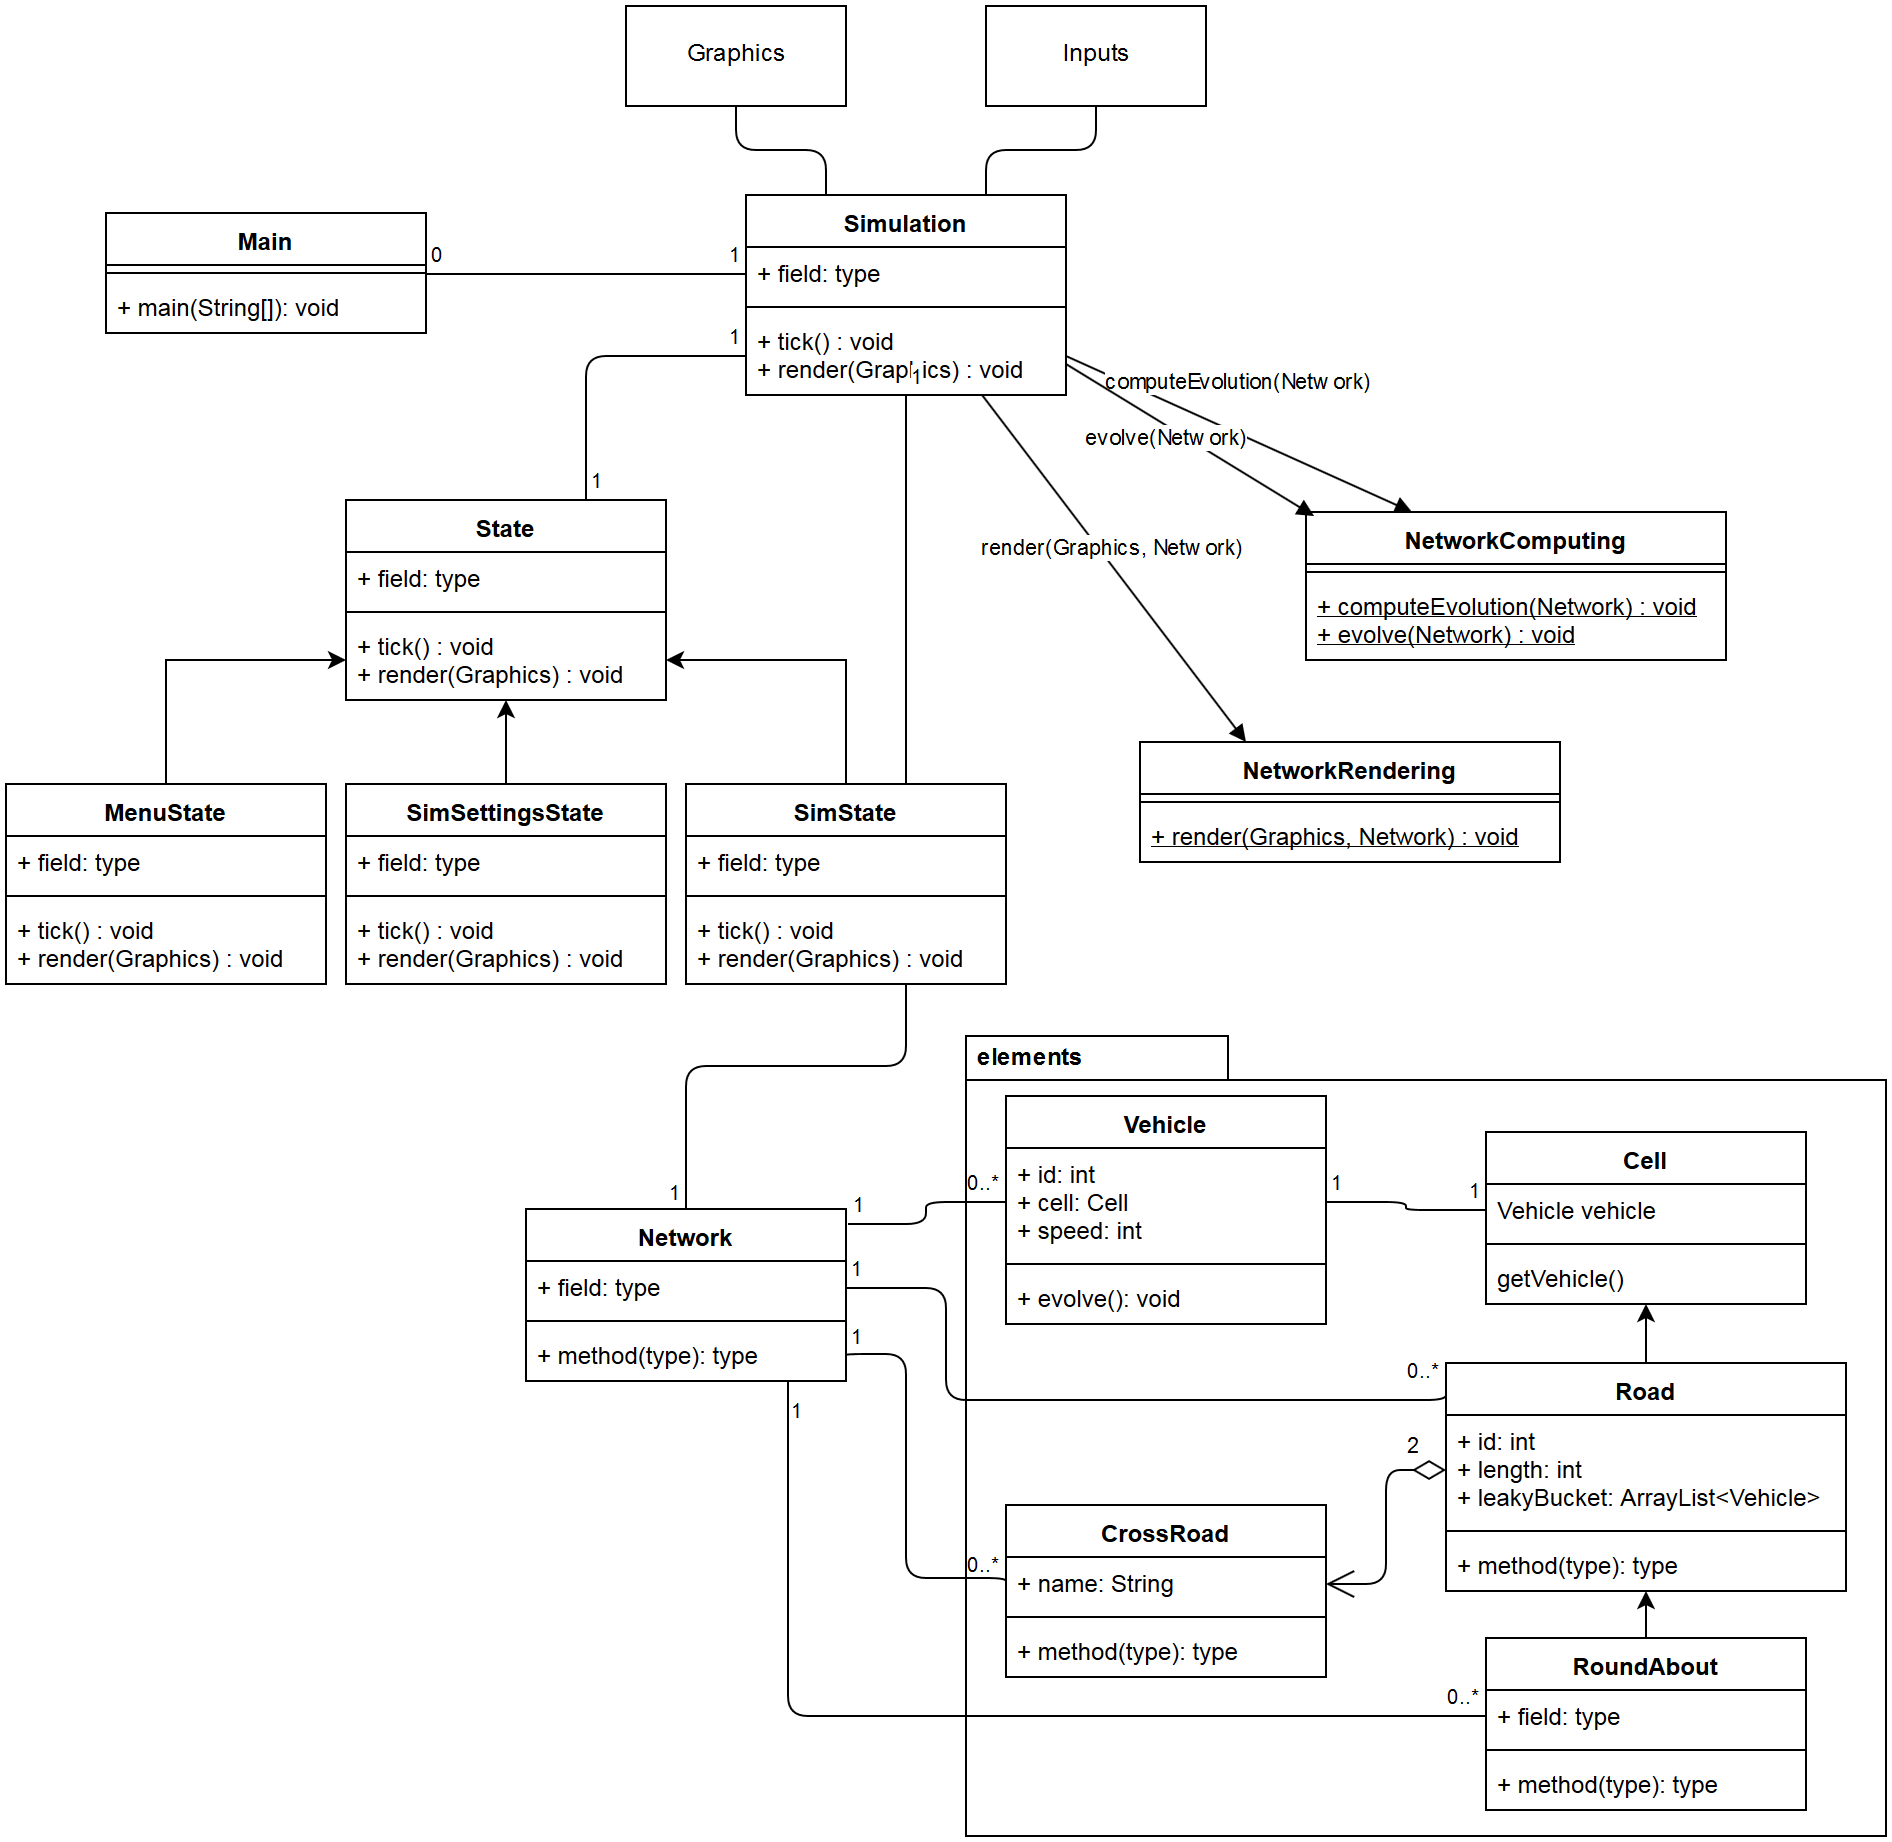
\includegraphics[width=15cm]{structure_diagram.png}
\caption{Diagramme de classe de la structure globale}
\label{imgGlobal}
\end{center}
\end{figure}

\paragraph{Simulation}

La classe principale \texttt{Main} se contente d'appeler une instance de \texttt{Simulation}. Cette classe gère le coeur du programme. Elle fait tourner la boucle qui maintient le programme en vie, tout en appelant les méthodes \texttt{tick()} et \texttt{render(Graphics)} de ses éléments 60 fois par seconde. La première méthode représente un tic d'horloge, permettant par exemple la mise à jour des éléments, tandis que la deuxième va appeler les méthodes graphiques nécessaires à l'interface. Elle reçoit aussi des classes du package \texttt{input} les informations nécessaires sur les actions de la souris et du clavier, et des classes du package \texttt{graphics} les méthodes utiles au rendu graphique à l'écran.

\paragraph{State}

La classe \texttt{Simulation} est également responsable de maintenir le état du programme parmis les états possibles : menu, options et simulation (voir section \ref{sctEtats}).

\paragraph{Network}

La classe \texttt{Network} représente le réseau routier au sens statique. Elle contient toutes les routes, ainsi que les véhicules, mais ne procèdent pas à l'évolution du modèle, ni à son rendu à l'écran, dont s'occupent respectivement les classes \texttt{NetworkComputing} et \texttt{NetworkRendering}. À l'opposé du \texttt{Network}, ces classes ne contiennent aucune information, mais fournissent des calculs pour l'évolution et des calculs pour le rendu. Ceci permet d'alléger fortement la classe \texttt{Network} qui est une classe complexe et centrale.

\subsubsection{\label{sctEtats}État du programme}

\begin{wrapfigure}[15]{r}{0.6\textwidth}
  \vspace{-1cm}

  \begin{center}
    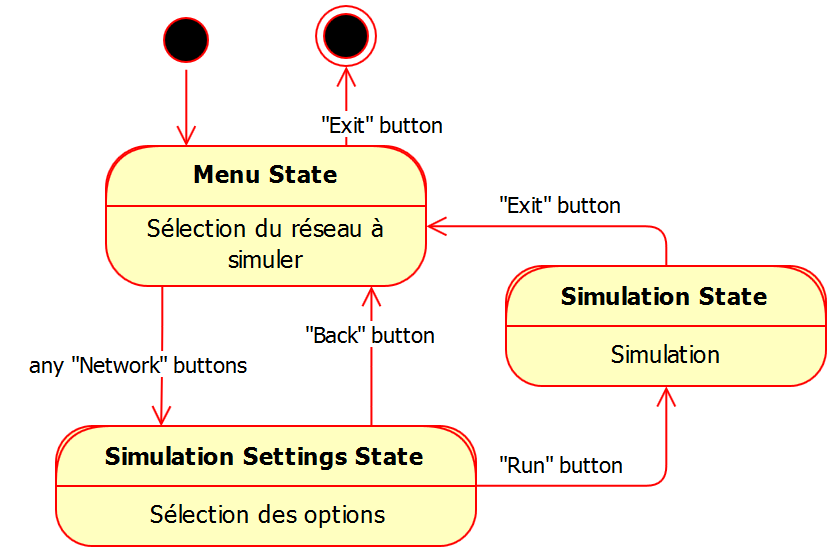
\includegraphics[width=0.55\textwidth]{states_diagram.png}
  \end{center}
  \caption{Diagramme d'état du programme}
  \label{imgStates}
\end{wrapfigure}

Le programme peut être dans un étant parmis les trois suivants : \texttt{Menu}, \texttt{Simulation Settings}, \texttt{Simulation}. Le premier état permet à l'utilisateur de choisir le réseau à simuler (réseau actuel ou scénarios alternatifs). Le deuxième permet quant à lui de modifier les données de simulation, c'est-à-dire le nombre de véhicules générés suivant leur provenance et leur destination. Les données par défaut sont les données recueillies par le CERN, et la DGT. Le dernier état lance la simulation du réseau et des données choisis par l'utilisateur. La figure \ref{imgStates} présente les états du programme et leur évolution possible.

La classe \texttt{Simulation} va appeler les méthodes \texttt{tick()} et \texttt{render(Graphics)} de l'état courant.

\subsubsection{Réseau routier}

\paragraph{Cellule}

Le quanta pour ce modèle est donc une cellule que nous implémentons dans une classe \texttt{Cell}. Tout autre élément (route, rond-point, carrefour) doit donc contenir une liste de ses cellules. Une cellule contient un lien vers la cellule suivante sur la route (\texttt{nextCell}), la cellule précédente (\texttt{previousCell}), ainsi qu'une cellule entrante symbolisant une route arrivant sur cette cellule (\texttt{inCell}), et une cellule sortant pour une route partant de cette cellule (\texttt{outCell}).

\paragraph{Route}

Une route contient une liste de cellules qui représentent les cellules de la route (\texttt{roadCells}), ainsi que sa longueur (\texttt{length}) et un éventuel ``leaky bucket'' (\texttt{leakyBucket}) qui est une liste de véhicules.

\paragraph{Rond-point}

De plus, un rond-point n'est en fait qu'une route enroulée sur elle-même, le rond-point est donc une spécialisation de la classe route, où la première et dernière cellule seront connectées entre elles.

\paragraph{Carrefour}

Un carrefour quant à lui doit contenir le lien avec les routes qui lui sont connectées. Il contient donc une liste des routes entrantes, une liste des routes sortantes, ainsi qu'une liste des cellules du carrefour.

\paragraph{Véhicule}

Finalement, un véhicule doit savoir sur quelle cellule il se situe, et une cellule doit aussi connaître le véhicule qui l'occupe. Le véhicule retient également en mémoire son emplacement pour le pas de temps suivant. La méthode \texttt{evolve()} permet de mettre à jour la position du véhicule lors d'un pas de temps.

\paragraph{Network}

\begin{figure}[!h]
\begin{center}
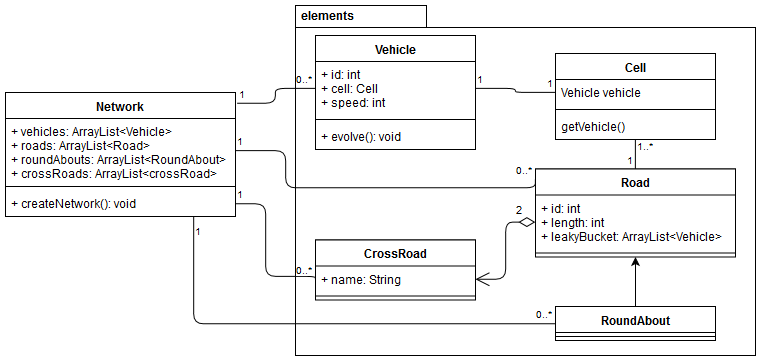
\includegraphics[width=13cm]{elements_diagram.png}
\caption{Diagramme de classe des éléments composants le réseau}
\label{imgElements}
\end{center}
\end{figure}

La classe \texttt{Network} doit utiliser tous les éléments afin de les combiner et mettre en place le réseau routier. Elle va non seulement créer les éléments et les garder en mémoire, mais aussi les connecter entre eux, ainsi que les placer visuellement sur l'écran. Elle contiendra donc une liste des véhicules, une liste des routes, une liste des rond-points et une liste des carrefours. Elle met à disposition plusieurs méthodes de la forme \texttt{create[...]Network()}, chacune permettant de générer un réseau différent. Cette classe reste cependant statique du point de vue de l'évolution : elle contient uniquement les éléments, et n'est pas responsable de les faire évoluer (voir section \ref{sctEvolution}). Elle fait uniquement office de conteneur d'information.

Ces premières réflexion nous amènent donc à considérer la structure présentée en figure \ref{imgElements}.

\subsubsection{Leaky Buckets}

Comme les routes entrants dans le modèle ne peuvent pas être de taille illimitée, chacune d'elle dispose d'un ``leaky bucket''. Au moment de la création d'un nouveau Véhicule en entrée de route, celle-ci est placée dans un leaky bucket appartenant à la route. Si le véhicule peut s'engager, alors le leaky bucket le dépose sur la première cellule de la route. Si cette cellule est occupée, le véhicule attend que celle-ci se libère. Ceci permet de simuler l'allongement d'une file de véhicules qui s'allongerait au-delà des limites du modèle, et permet de voir les impacts de embouteillages au-delà des abords directs du CERN.

\subsection{Pré-processing}

Avant de lancer la simulation, il est nécessaire de mettre plusieurs éléments en place pour celle-ci.

\subsubsection{Trajets}

\begin{wrapfigure}[17]{r}{0.3\textwidth}
  \begin{center}
    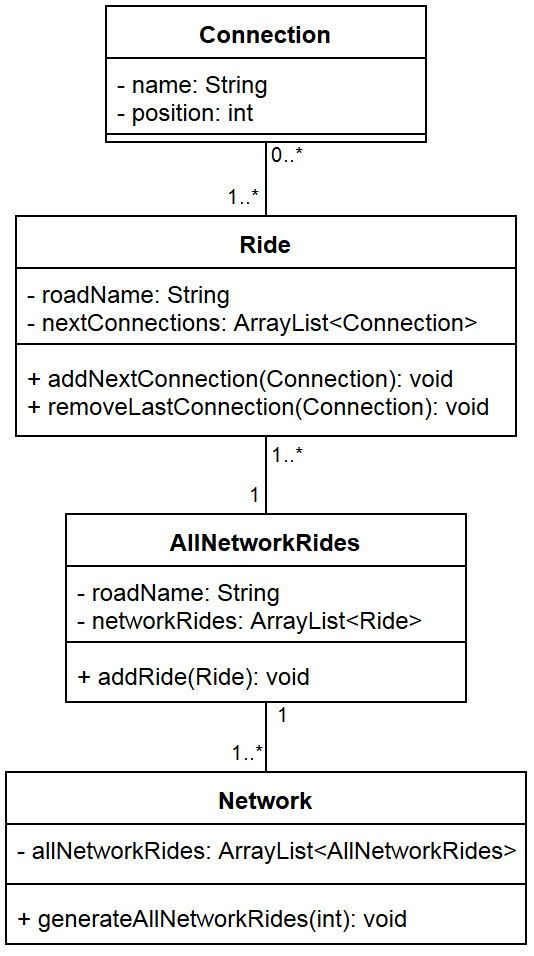
\includegraphics[width=0.25\textwidth]{rides_diagram.png}
  \end{center}
  \caption{Diagramme de classe des trajets}
  \label{imgRides}
\end{wrapfigure}

Un des éléments importants du modèle est de donner à chaque véhicule un trajet défini. Nous devons en effet nous assurer de maîtriser le trajet de chaque véhicule, ainsi que la génération de nouveaux véhicules suivant les données récoltées par le CERN.

\paragraph{Connection}

Cette classe représente la connexion de la cellule indexée par \texttt{position} à une autre route nommée \texttt{name}.

\paragraph{Ride}

Cette classe représente un trajet possible d'un véhicule à partir d'une route étiquetée par \texttt{roadName}. Elle contient une liste de \texttt{Connection} permettant au véhicule de savoir à quelle cellule se trouve la sortie qu'il doit emprunter.

\paragraph{AllNetworkRides}

Cette classe représente tous les trajets possibles d'un véhicule à partir d'une route étiquetée par \texttt{roadName}. Ces trajets sont stockés dans une liste de \texttt{Ride}.

\paragraph{Network}

Cette classe utilise finalement une liste de \texttt{AllNetworkRides} lui permettant de connaître tous les trajets possibles pour chacune de ses routes. Au lancement de la simulation, la méthode \texttt{generateAllNetworkRides()} permettra de générer tous les trajets du réseau.

\subsubsection{Données}

Au moment du choix d'un des réseaux dans le menu, les données récoltées par le CERN et la DGT sont placées dans les options de la simulation. Une fois que les valeurs ont été choisies par l'utilisateur, la classe \texttt{DataManager} va implémenter ces données au réseau. A chaque \texttt{Ride} est attribué une liste d'entiers représentant le nombre de véhicule à générer à chaque heure de la journée, pour ce trajet. Ceci permet donc de savoir pour chaque route, la probabilité de générer un nouveau véhicule sur cette route, ainsi que le trajet à lui assigner.

\subsubsection{Pré-proccesing graphique}

Afin d'être sûr de rendre le programme aussi léger que possible, l'image du réseau est calculé avant la simulation et placée en mémoire. Seuls les véhicules et les boutons sont recalculés à chaque pas de temps. Ceci permet de changer les options de visualisation quasi instantanément et assure une simulation aussi rapide que possible.

\subsection{\label{sctEvolution}Évolution du modèle}

L'évolution du réseau est effectué du point de vue des véhicules par la classe \texttt{NetworkComputing}.

\paragraph{computeEvolution(Network)}

Dans un premier temps, la méthode génère les nouveaux véhicules pour les routes entrants dans le modèle. La méthode met ensuite à jour les feux des carrefours.

La méthode passe en revu les véhicules un par un, en enregistrant pour chacun l'état qu'il devra avoir au pas de temps suivant dans l'attribut \texttt{nextPlace} des cellules. Les règles de la simulation sont les suivantes :

\begin{enumerate}
\item Si la cellule devant le véhicule est occupée, le véhicule ne se déplace pas.
\item Si la cellule devant le véhicule est libre mais celle d'après occupée, et que le véhicule à une vitesse de 2, celui-ci décélère : il avance d'une case.
\item Si les deux cellules devant le véhicule sont libres, le véhicule peut accélérer de 1.
\item Un véhicule ne peut s'engager sur un rond-point que si aucun véhicule ne doit décélérer pour lui laisser la place.
\item Si un véhicule arrive à un carrefour, il ne s'engage que si le feu est vert pour lui.
\item Si une route se termine en arrivant sur une autre route, le véhicule laisse la priorité aux véhicules venant de gauche.
\item Si un véhicule arrive en bout de route et qu'aucune autre structure n'est attachée, alors le véhicule quitte le réseau et est détruit.
\end{enumerate}

\paragraph{evolve(Network)}

Une fois que toutes les nouvelles positions des véhicules ont été calculées, alors seulement le réseau est mis-à-jour. Les véhicules sont passé en revue et leur position \texttt{cell} devient celle contenue dans \texttt{nextPlace}. Le réseau évolue donc entièrement pas à pas, chaque véhicule avance en même temps que les autres. Ceci évite des problèmes de simulation dans le cas où les véhicules seraient déplacés un par un.

\newpage

\section{Prise en main}

\emph{Nous allons passer en revue les fonctions principales offertes par le code. Pour des informations plus détaillées, nous vous invitons à consulter le manuel\footnote{https://github.com/lutzilutz/TraficCERN/wiki}.}\newline

\subsection{Création du réseau}

La création d'un réseau se fait dans la classe \texttt{Network}, dans l'une des méthodes appelées dans la structure \texttt{switch} du constructeur. En effet, à l'instanciation du réseau, il faut donner en paramètre un entier, qui correspond au réseau choisi parmis les possibilités (le réseau actuel du CERN est déclaré dans \texttt{createRealNetwork()}).

\subsubsection{Création d'une route}

Nous voulons créer une route nommée ``route'', orientée à 270$\degree$ et sortant d'un rond point nommé ``rondPoint''.

\begin{lstlisting}[language=Java]
Road route = new Road(this, 15, "route"); // instanciation
route.setStartPositionFrom(rondPoint, 7); // position de depart
route.setDirection(270); // direction 0=north, 90=east, ...
roads.add(route); // ajout de la route au reseau
rondPoint.connectTo(route, 7); // connexion
\end{lstlisting}

Il faut instancier la route avec sa longueur en nombre de cellules, ici 15, ainsi que son nom qui devra être unique dans le réseau, ici \texttt{route}. Nous pouvons ensuite placer la route par rapport à un autre élément. Ici, le début de la route sera placée par rapport à la $8^e$ cellule (indice 7). Il faut aussi lui donner sa direction, ici à l'ouest, et finalement ajouter la route créer à la liste des routes, \texttt{roads}. La dernière étape consiste à connecter les cellules ensemble, par la méthode \texttt{connectTo()}. Il est important de noter que l'indice de la connexion doit être le même que l'indice du placement (la valeur \texttt{7} des lignes 2 et 5).

\subsubsection{Virages}

En reprenant la route du point précédent, nous pouvons ajouter des cassures dans la route pour symboliser un virage.

\begin{lstlisting}[language=Java]
route.addPoint(new Point(4,0)); // cassure a la cellule 4
route.addPoint(new Point(9,90)); // cassure a la cellule 9
\end{lstlisting}

Avec ce code ajouté à la suite du précédent, nous spécifions qu'à la case d'indice 4, la route prend une direction de 0$\degree$ ce qui correspond au plein nord. Nous ajoutons ensuite une deuxième cassure à la cellule d'indice 9 où la route se dirige ensuite à 90$\degree$ soit à l'est. La route dessine donc un ``C''.

\subsubsection{Création d'un rond-point}

Nous voulons maintenant créer un rond-point que nous appellerons ``rondPoint''.

\begin{lstlisting}[language=Java]
RoundAbout rondPoint = new RoundAbout(this, 48, "rondPoint"); // instanciation
rondPoint.setX(0); // position en X
rondPoint.setY(0); // position en Y
rondPoint.setDirection(0); // direction
roundAbouts.add(rondPoint); // ajout du rond-point au reseau
\end{lstlisting}

Nous instancions le rond-point avec sa longueur ainsi que son nom, de manière identique que les routes. Si le rond-point est le premier élément placé, celui-ci peut être placé à la valeur désiré, le point $(x=0,y=0)$ correspondant au coin haut gauche de l'écran. La direction est placée à 0 signifiant que la cellule parfaitement au nord du rond-point est la cellule d'indice 0 (indice croissant dans le sens anti-horaire). Finalement nous ajoutons le rond-point à la liste des rond-points du réseau.

\subsection{Ajout des données}

\subsubsection{Probabilité uniforme sur la journée}

L'ajout de données se fait par la classe \texttt{DataManager}. La méthode \texttt{applyDataToRides()} transfère les données sur les trajets, et \texttt{applyRidesToRoads()} fait la somme des probabilités des trajets et les transfère sur les routes. Vous pouvez entrer les valeurs manuellement comme suit : 

\begin{lstlisting}[language=Java]
for (Ride ride: n.getAllRides("routeStart").getNetworkRides()) {
	if (lastRoadIs(ride, "routeEnd")) {
		ride.setFlow(50); // nombre de vehicules a generer
	}
}
\end{lstlisting}

La boucle de la première ligne va itérer sur tous les \texttt{Ride} dont le point de départ est \texttt{routeStart}, c'est à dire sur tous les trajets possibles partant de cette route. La condition de la deuxième ligne va sélectionner seulement le trajet dont le point d'arrivée est \texttt{routeEnd}. Nous pouvons ensuite entrer la valeur que nous désirons, qui correspond à un nombre de véhicule à générer avec ce trajet par heure.

\subsubsection{Probabilité hétérogène}

\begin{lstlisting}[language=Java]
r.setFlow(20); // probabilite uniforme
r.setFlow(7, 8, 300); // heures de pointes
\end{lstlisting}

Si nous souhaitons préciser un taux de création de véhicule différent suivant les heures de la journée, nous pouvons utiliser une autre version de \texttt{setFlow()}. Celle-ci permet de préciser d'avoir un certain taux entre 2 heures de la journée, ici un taux de 300 de 7 à 8 heures (60 minutes).

Il est aussi possible d'utiliser des variables du code plutôt que de rentrer manuellement les données, ce que nous avons fait dans notre code pour avoir un lien entre les données et les options du menu.
\vspace{0.5cm}
\subsubsection{Compteurs}

Après la mise en place d'une route, nous pouvons activer un compteur sur celle-ci.

\begin{lstlisting}[language=Java]
route.setCounter(0.3); // compteur a 30% de la longueur de la route
\end{lstlisting}

Cette ligne va activer le compteur de la \texttt{route}, à une distance de 30\% de la longueur de la route, en partant de son commencement. Le compteur affiche ensuite dans l'interface le nombre de véhicule qui passe par ce point par minute. Le compteur est actualisé chaque minute, avec la formule

\begin{equation*}
R_{i+1} = R_i + (1-\alpha) \cdot C_i
\end{equation*}

Où les $R_i$ sont les débits à un instant $i$ et $C_i$ le nombre de véhicules passé entre l'instant $i$ et $i+1$, et $\alpha = 1/8$ afin d'avoir une mise-à-jour rapide.

\subsection{Extraction des données}

Les données sont automatiquement sauvegardée dans un fichier texte à la racine du programme Java. Afin de rajouter aux fichiers le compteur que nous avons créée, nous devons modifier la méthode \texttt{writeData(Network)} de la classe \texttt{NetworkComputing}.

\begin{lstlisting}[language=Java]
public static void writeData(Network n) {
	Utils.writeData(n.getSimulation().getSimState().getTime() + " ");
	Utils.writeData(Integer.toString(n.selectARoad("x").getVehicleCounter().getCounter())+" ");
	Utils.writeData(Integer.toString(n.selectARoad("y").getVehicleCounter().getCounter())+"\n");
}
\end{lstlisting}

Si nous avons ajouté deux compteurs, l'un à une route nommée \texttt{x} et l'autre à une route nommée \texttt{y}, il nous suffit de rajouter les lignes 3 et 4 pour obtenir les données à chaque minute de la simulation. La ligne 2 écrit la date et l'heure dans la simulation en début de ligne, suivie par les valeurs des compteurs séparés par des espaces.

Nous devons également changer l'en-tête du fichier de données, grâce à la classe \texttt{Utils}. 

\begin{lstlisting}[language=Java]
public static void initData() {
	[...]
	data.print("Time CounterX CounterY\n");
}
\end{lstlisting}

Cette ligne sera la première imprimée en début de simulation, elle correspond donc à l'en-tête de chacune des colonnes. Les 3 appels à \texttt{writeData(Network)} correspondent donc aux trois en-têtes ci-dessus.

\newpage

\section{Évolution du projet}

La première remarque que nous pouvons faire est que nous avons sous-estimé la quantité de travail nécessaire afin d'atteindre ces objectifs. Le modèle étant simple, et la simulation ne s'intéressant qu'à une dizaine de route, nous avons pensé le projet plus court que ce qu'il s'est finalement avéré. Sur la table \ref{tabTemps} se trouve un résumé de la quantité écrite et du temps estimé.

\begin{table}[h!]
\begin{center}
\begin{tabular}{|l|c|c|c|}
\hline
 & addition & suppression & total\\ \hline
\#lignes & 13'000 & 7'000 & 6'000\\ \hline
\#lignes par minute & 3 & 6 & - \\ \hline\hline
temps (minute) & 4'333 & 1'1167 & 5'500\\ \hline
temps par étudiant (heure) & 36 & 10 & 46\\ \hline
\end{tabular}
\end{center}
\caption{Temps estimé par rapport au nombre de lignes écrites}
\label{tabTemps}
\end{table}

Ce résultat ne prends pas en compte le temps que nous avons passé à discuter, par des réunions, des appels, ou des messages écrits. La durée totale de ces discussions dépasse facilement 20 heures. Nous arrivons donc à un total par étudiant de 66 heures de travail total.

\end{document}
